\documentclass[twocolumn]{sintr}
\setlength\parindent{0pt}
\usepackage{lipsum}  

% 
% Volume, issue, year, page range
\articleinformation{Vol xx, No x, xxxx, xx–xx} 
% 
% Truncated volume, issue, page range
\articleinformationtruncated{xx(x): xx–xx} 
%
% BSMS Thesis / Winter Project / Summer Project / Project
\articletype{lab report} 
%
% \submitted{20 January 2023} 
%
% Article title
\title{JiaShua}
%
\articleshorttile{Give a short Title of the Project/Thesis}
% Author(s)
%
\author{Nan Jia}
\author{Joshua Rollins}
%
% Author name(s) as they should appear in the header
% \authorheader{Short Names of Authors}
%
%
%% ==>
%
%--------------------------------------------------
% Author(s) affiliations                      -->  
%--------------------------------------------------
%
%% ==>

%
\affil[1]{The graduate center, CUNY}
%% ==>

% Corresponding author
\affil[$\mbox{*}$]{Corresponding author: \href{mailto:sjena@iisermohali.ac.in}{sjena@iisermohali.ac.in}}
%
% Abstract
\abstract{The abstract introduces the reader to the background and objective of the work in a few sentences, the methods used in 3-10 sentences, the principal results in a few sentences, and conclusions in a line. It should be concise and written in 300-500 words in a single paragraph, or better to avoid abbreviations and citations. }

% Keywords
\keywords{Alphabetical order \\ 
Maximum five keywords \\
Avoid terms already in \\
\hphantom{} the title}

% PDF metadata (authors ignore)
\makeatletter
% \hypersetup{pdftitle={\@title},pdfauthor={\authorheader}, pdfkeywords={\keywords}, pdfsubject={\abstract}}
\makeatother

\makeatletter
\def\MT@warn@unknown{}
\makeatother



\begin{document}
\setcounter{page}{1}
\maketitle

\thispagestyle{firststyle}
%\linenumbers % Add line numbers

\section{Introduction}

This section should briefly explain the background of the study, provide a short review of the pertinent literature, state the originality or novelty of the research, and state the research objectives.

\section{Subsequent Sections}

Write down the report and add enough sections accordingly.

\section{Various Commands}
\subsection{Tables}

Size a table to fit in a single column (Table \ref{tab:1}) or across two columns (Table \ref{tab:2}). Avoid large tables (i.e., those that fit more than a single page), unless necessary.

Every table and figure should be cited in the text in numerical order (i.e., Table 2 cannot be cited before Table 1). Place table footnotes below the table, indicating them with superscripted lowercase letters or asterisks (for significance values and other statistical data).

%
%
%---------------------------------------------
%

\subsubsection{Table captions}
Every table should have a concise but clear caption to explain its main components independently from the text. If the table contains previously published material, cite the original source at the end of the caption. If the results are expressed as a percentage, state the absolute value(s) that correspond to 100\%.

\begin{table}[b]
  	\centering\footnotesize\sffamily
  	\caption{Example single-column table.}
  	\begin{tableminipage}{\linewidth}
    	\begin{tabularx} {\linewidth}{XXX}
			\toprule
            Column 1\textsuperscript{a} & Column 2 & Column 3  \\            
	    	\midrule
             1 &  1 &  1 \\
             2 &  2 &  2 \\
             3 &  3 &  3 \\
             4 &  4 &  4 \\
             5 &  5 &  5 \\
            \bottomrule
    	\end{tabularx}
        \label{tab:1}
        \vskip0pt
        \textsuperscript{a}Example footnote.
  	\end{tableminipage}
\end{table}

\begin{table*}[t]
  	\centering\footnotesize\sffamily
  	\caption{Example double-column table.}
  	\begin{tableminipage}{\linewidth}
    	\begin{tabularx} {\linewidth}{XXXXXX}
			\toprule
            Column 1 & Column 2 & Column 3 & Column 4 & Column 5 & Column 6 \\            
	    	\midrule
             11 &  12 &  13 &  14 &  15 &  16 \\
             21 &  22 &  23 &  24 &  25 &  26 \\
             31 &  32 &  33 &  34 &  35 &  36 \\
             41 &  42 &  43 &  44 &  45 &  46 \\
             51 &  52 &  53 &  54 &  55 &  56 \\
            \bottomrule
    	\end{tabularx}
        \label{tab:2}
  	\end{tableminipage}
\end{table*}

\subsection{Figures}

Ensure that the figure will fit into either one column (Figure \ref{fig:1}) or two columns (Figure \ref{fig:1}). Images should be of sufficiently high resolution to be easily viewable when printed or on high-resolution screens (minimum of 300 dpi).

Every figure should be cited in the text in numerical order (i.e. Figure 2 cannot be cited before Figure 1). Figures should be referred to as "Figure" not "Fig." Denote figure parts with lowercase letters (e.g. Figure 1a, Figure 1b).

\subsubsection{Figure formatting}

Photographs must have internal scale markers and symbols; arrows or letters should contrast greatly with the background. Fira Sans is the recommended typeface for text within figures (if you don’t have it installed on your computer, you can download it from Google Fonts). Otherwise, a sans-serif such as Open Sans or Helvetica may be used. Where photographs of gel, autoradiograms, and so on have been processed to enhance their quality, this should be stated.


\lipsum[1]

\subsubsection{Figure captions}

Every figure should have a concise but clear caption to explain its main components independently from the text. If the figure contains previously published material, cite the source at the end of the caption.

\begin{figure}[!b]
	\centering
	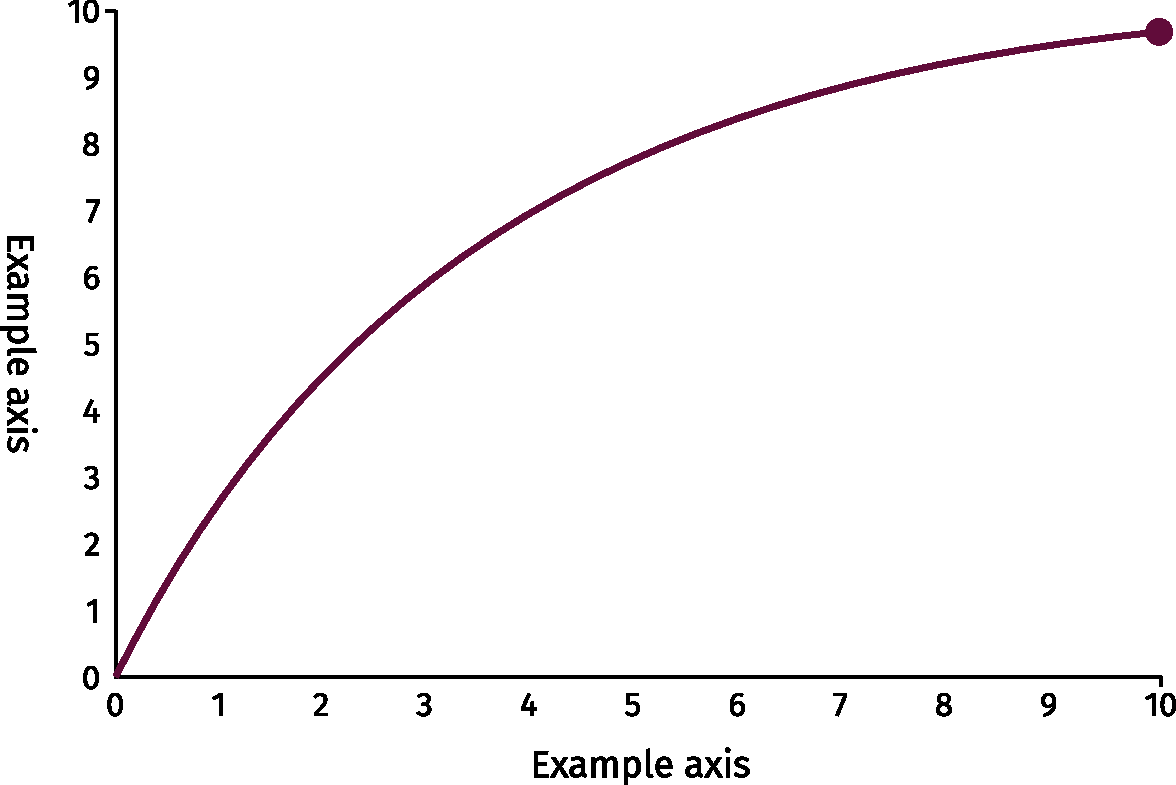
\includegraphics[width=\linewidth]{Figure1.pdf}
	\caption{Example figure caption for a single-column image.}
	\label{fig:1}
\end{figure}

\lipsum[1]


\section{Conclusion}

Present the study's main conclusions, along with their implications for future research or science and technology policy in the ASEAN region.

\section*{Acknowledgement}

Please acknowledge anyone who contributed to the research or the writing of the manuscript, as well as any funding or grants received in support of it. The names of funding organizations should be written in full, along with the grant numbers, if available. Examples of individuals you should acknowledge include people who assisted with study design or analysis, or guidance through a study area, or who provided advice on the language, edited, or proofread the article.

\lipsum[2-10]

\section*{AUTHORS’ CONTRIBUTIONS}

Each author’s contribution to the research and manuscript should be noted, using only their initials to indicate their names. For example, “MP, FW designed the study. MP, LS carried out the laboratory work. MP, FW, LS, DN analyzed the data. MP, FW, DN wrote the manuscript. All authors read and approved the final version of the manuscript.”

\section*{COMPETING INTERESTS}

All competing interests—financial, professional, or personal relationships relevant to the submitted work—must be declared. This should be clearly stated if a funding source contributed to the manuscript's design, data collection, analysis, or writing or the decision to submit it to AJSTD. If one or more authors have any form of—past or present—relationship with AJSTD, the extent of this relationship must be described. This must also be clearly stated if one or more authors work or have worked for an organization that may benefit from the article's publication. Please read AJSTD’s Publication Ethics statement to understand why it is essential to acknowledge any competing interests.

\lipsum[1]

\lipsum[2-14]

\section*{References and Citations}
Please put the references in a separate file, like ref. Bib like this template. You must use the Bibtex format. Preparing the Bibtex reference format is very simple; you can use inspire hep.net  to get the reference in BibTex format. Then use \cite{aa} to cite the references  \cite{bb}. 

\bibliography{ref}

\atColsEnd{\vfill}

\end{document}